\begin{figure}[!htbp]
	\centering
	\resizebox{0.85\textwidth}{!}{%
		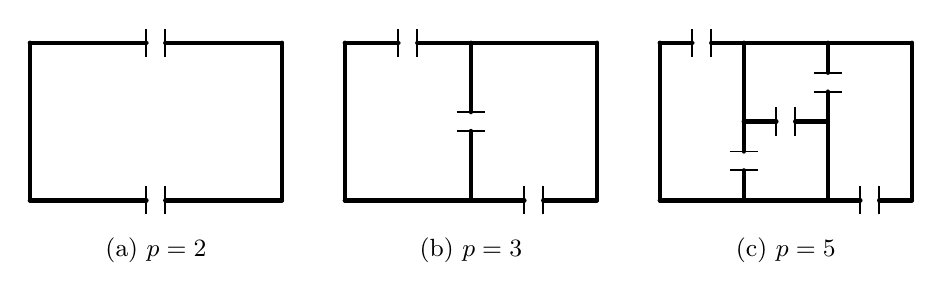
\begin{tikzpicture}[
			>=stealth, line width=0.8pt,
			trave/.style={line width=1.6pt, line cap=round,
				line join=round, black},
			taglio/.style={line width=0.7pt, black}]
			
			%% ===============================================================
			%% PANNELLO (a) — trave biconnessa: rettangolo (p = 2)
			%% ===============================================================
			\begin{scope}[xshift=0cm, yshift=0cm]
				
				\def\W{3.2}      %% larghezza del rettangolo
				\def\H{2.0}      %% altezza
				\def\dt{0.12}    %% mezza-larghezza dell'interruzione di trave
				\def\el{0.18}    %% mezza-lunghezza del trattino trasversale
				
				%% Posizione dei due tagli:
				%% uno sul lato superiore in W/2, uno sul lato inferiore in W/2
				\pgfmathsetmacro{\xTa}{\W*0.5}    %% taglio superiore
				\pgfmathsetmacro{\xTb}{\W*0.5}    %% taglio inferiore
				
				%% --- lato superiore: due segmenti, interrotto in xTa ---
				\draw[trave] (0,\H) -- ({\xTa-\dt},\H);
				\draw[trave] ({\xTa+\dt},\H) -- (\W,\H);
				%% trattini trasversali del taglio superiore
				\draw[taglio] ({\xTa-\dt},{\H-\el}) -- ({\xTa-\dt},{\H+\el});
				\draw[taglio] ({\xTa+\dt},{\H-\el}) -- ({\xTa+\dt},{\H+\el});
				
				%% --- lato inferiore: due segmenti, interrotto in xTb ---
				\draw[trave] (0,0) -- ({\xTb-\dt},0);
				\draw[trave] ({\xTb+\dt},0) -- (\W,0);
				%% trattini trasversali del taglio inferiore
				\draw[taglio] ({\xTb-\dt},{-\el}) -- ({\xTb-\dt},{\el});
				\draw[taglio] ({\xTb+\dt},{-\el}) -- ({\xTb+\dt},{\el});
				
				%% --- lati corti, integri ---
				\draw[trave] (0,0) -- (0,\H);
				\draw[trave] (\W,0) -- (\W,\H);
				
				%% --- etichetta pannello ---
				\node[below=10pt, font=\small] at (\W/2,0) {(a) $p=2$};
			\end{scope}
			
			%% ===============================================================
			%% PANNELLO (b) — triconnessa: + un setto verticale (p = 3)
			%% ===============================================================
			\begin{scope}[xshift=4cm, yshift=0cm]
				
				\def\W{3.2}      %% larghezza del rettangolo
				\def\H{2.0}      %% altezza
				\def\dt{0.12}    %% mezza-larghezza dell'interruzione
				\def\el{0.18}    %% mezza-lunghezza del trattino trasversale
				
				%% Posizione dei tre tagli
				\pgfmathsetmacro{\xTa}{\W*0.25}   %% sup, sinistra del setto
				\pgfmathsetmacro{\xTb}{\W*0.75}   %% inf, destra del setto
				\pgfmathsetmacro{\xS}{\W*0.50}    %% ascissa setto verticale
				\pgfmathsetmacro{\yTs}{\H*0.50}   %% taglio sul setto, a meta' altezza
				
				%% --- lato superiore: interrotto in xTa, setto in xS (continuo) ---
				\draw[trave] (0,\H) -- ({\xTa-\dt},\H);
				\draw[trave] ({\xTa+\dt},\H) -- (\W,\H);
				\draw[taglio] ({\xTa-\dt},{\H-\el}) -- ({\xTa-\dt},{\H+\el});
				\draw[taglio] ({\xTa+\dt},{\H-\el}) -- ({\xTa+\dt},{\H+\el});
				
				%% --- lato inferiore: interrotto in xTb ---
				\draw[trave] (0,0) -- ({\xTb-\dt},0);
				\draw[trave] ({\xTb+\dt},0) -- (\W,0);
				\draw[taglio] ({\xTb-\dt},{-\el}) -- ({\xTb-\dt},{\el});
				\draw[taglio] ({\xTb+\dt},{-\el}) -- ({\xTb+\dt},{\el});
				
				%% --- lati corti, integri ---
				\draw[trave] (0,0) -- (0,\H);
				\draw[trave] (\W,0) -- (\W,\H);
				
				%% --- setto verticale interno, interrotto in yTs ---
				\draw[trave] (\xS,0) -- (\xS,{\yTs-\dt});
				\draw[trave] (\xS,{\yTs+\dt}) -- (\xS,\H);
				%% trattini orizzontali del taglio sul setto
				\draw[taglio] ({\xS-\el},{\yTs-\dt}) -- ({\xS+\el},{\yTs-\dt});
				\draw[taglio] ({\xS-\el},{\yTs+\dt}) -- ({\xS+\el},{\yTs+\dt});
				
				%% --- etichetta pannello ---
				\node[below=10pt, font=\small] at (\W/2,0) {(b) $p=3$};
			\end{scope}
			
			%% ===============================================================
			%% PANNELLO (c) — p = 5: + due setti verticali + uno orizzontale
			%% ===============================================================
			\begin{scope}[xshift=8cm, yshift=0cm]
				
				\def\W{3.2}      %% larghezza del rettangolo
				\def\H{2.0}      %% altezza
				\def\dt{0.12}    %% mezza-larghezza dell'interruzione
				\def\el{0.18}    %% mezza-lunghezza del trattino trasversale
				
				%% Ascisse dei due setti verticali interni: in W/3 e 2W/3
				\pgfmathsetmacro{\xSa}{\W/3}      %% setto verticale sinistro
				\pgfmathsetmacro{\xSb}{2*\W/3}    %% setto verticale destro
				\pgfmathsetmacro{\yO}{\H*0.50}    %% quota del setto orizzontale
				
				%% Posizione dei cinque tagli
				\pgfmathsetmacro{\xTa}{\W/6}      %% taglio 1: sup, sx del setto sx
				\pgfmathsetmacro{\xTb}{5*\W/6}    %% taglio 2: inf, dx del setto dx
				\pgfmathsetmacro{\yTc}{\H*0.25}   %% taglio 3: setto sx, sotto
				\pgfmathsetmacro{\yTd}{\H*0.75}   %% taglio 4: setto dx, sopra
				\pgfmathsetmacro{\xTe}{\W*0.50}   %% taglio 5: setto orizz., centro
				
				%% --- lato superiore: interrotto in xTa, attraversato dai due setti ---
				\draw[trave] (0,\H) -- ({\xTa-\dt},\H);
				\draw[trave] ({\xTa+\dt},\H) -- (\W,\H);
				\draw[taglio] ({\xTa-\dt},{\H-\el}) -- ({\xTa-\dt},{\H+\el});
				\draw[taglio] ({\xTa+\dt},{\H-\el}) -- ({\xTa+\dt},{\H+\el});
				
				%% --- lato inferiore: interrotto in xTb ---
				\draw[trave] (0,0) -- ({\xTb-\dt},0);
				\draw[trave] ({\xTb+\dt},0) -- (\W,0);
				\draw[taglio] ({\xTb-\dt},{-\el}) -- ({\xTb-\dt},{\el});
				\draw[taglio] ({\xTb+\dt},{-\el}) -- ({\xTb+\dt},{\el});
				
				%% --- lati corti, integri ---
				\draw[trave] (0,0) -- (0,\H);
				\draw[trave] (\W,0) -- (\W,\H);
				
				%% --- setto verticale sx: interrotto in yTc (sotto) ---
				\draw[trave] (\xSa,0) -- (\xSa,{\yTc-\dt});
				\draw[trave] (\xSa,{\yTc+\dt}) -- (\xSa,\H);
				\draw[taglio] ({\xSa-\el},{\yTc-\dt}) -- ({\xSa+\el},{\yTc-\dt});
				\draw[taglio] ({\xSa-\el},{\yTc+\dt}) -- ({\xSa+\el},{\yTc+\dt});
				
				%% --- setto verticale dx: interrotto in yTd (sopra) ---
				\draw[trave] (\xSb,0) -- (\xSb,{\yTd-\dt});
				\draw[trave] (\xSb,{\yTd+\dt}) -- (\xSb,\H);
				\draw[taglio] ({\xSb-\el},{\yTd-\dt}) -- ({\xSb+\el},{\yTd-\dt});
				\draw[taglio] ({\xSb-\el},{\yTd+\dt}) -- ({\xSb+\el},{\yTd+\dt});
				
				%% --- setto orizzontale: da xSa a xSb, interrotto in xTe ---
				\draw[trave] (\xSa,\yO) -- ({\xTe-\dt},\yO);
				\draw[trave] ({\xTe+\dt},\yO) -- (\xSb,\yO);
				\draw[taglio] ({\xTe-\dt},{\yO-\el}) -- ({\xTe-\dt},{\yO+\el});
				\draw[taglio] ({\xTe+\dt},{\yO-\el}) -- ({\xTe+\dt},{\yO+\el});
				
				%% --- etichetta pannello ---
				\node[below=10pt, font=\small] at (\W/2,0) {(c) $p=5$};
			\end{scope}
			
		\end{tikzpicture}
	}
	\caption{Travi pluriconnesse di grado crescente. In
		ciascun pannello i $p$ tagli trasversali necessari
		a separare la linea d'asse in due tratti
		monoconnessi sono indicati dall'interruzione della
		linea fra due trattini paralleli.
		(a)~Trave biconnessa ($p = 2$): la linea
		d'asse è chiusa; due tagli la separano in due
		tratti monoconnessi. L'iperstaticità interna è
		$3(p-1) = 3$.
		(b)~Trave triconnessa ($p = 3$): un setto
		verticale interno introduce un secondo anello;
		tre tagli separano la trave in due tratti
		monoconnessi. L'iperstaticità interna è
		$3(p-1) = 6$.
		(c)~Trave pluriconnessa con $p = 5$: due setti
		verticali interni e un setto orizzontale corto
		che li collega creano quattro anelli; cinque
		tagli separano la trave in due tratti monoconnessi.
		L'iperstaticità interna è $3(p-1) = 12$.
		Il grado di connessione dipende solo dalla
		topologia della linea d'asse, indipendentemente
		dai vincoli esterni (qui assenti).}
	\label{fig:gradi_connessione}
\end{figure}
